\documentclass[12pt,a4paper]{article}

% Packages
\usepackage{amsmath}
\usepackage{graphicx}
\usepackage{float}
\usepackage{hyperref}
\usepackage{times}
\usepackage{booktabs}
\usepackage{geometry}
\geometry{margin=1in}

% Document
\begin{document}

% Title, Author, Date
\title{Tugas TBO 6}
\author{Davidson Rafael Krisman Nugroho - 412024030}
\date{\today}
\maketitle

% Soal
\section*{Soal}
Di Kutub Selatan terdapat enam binatang yang terdiri dari induk pinguin, anak pinguin, induk
singa laut, anak singa laut, induk beruang kutub dan anak beruang kutub. Semua binatang ini
hendak menyeberang ke gunung es pada sisi lainnya. Diantara dua gunung es ini terdapat balok
es yang hanya bisa ditempati untuk dua binatang saja. Namun terdapat suatu masalah yaitu
anak binatang tidak boleh ditinggal bersama induk binatang yang berlainan jenis dan singa laut
harus menjadi yang pertama sampai di sisi lainnya karena anak singa laut sedang terluka
sehingga harus cepat sampai di kelompoknya. Bantulah mereka untuk menyeberang ke gunung es pada sisi lainnya.

\section*{Jawaban}
Untuk menyelesaikan masalah ini, kita dapat menggunakan pendekatan langkah demi langkah untuk memeastikan bahwa 
semua binatang dapat menyeberang dengan aman sesuai dengan aturan yang diberikan. Dan saya juga memberikan kode 
python untuk mensimulasikan proses penyeberangan ini, serta JFLAP untuk memvisualisasikan solusi. Jawaban lengkapnya ada di halaman berikutnya.

\newpage
\subsection*{Penjelasan}

Untuk dapat memahami solusi dari masalah ini, kita perlu memahami aturan-aturan yang ada:
\begin{itemize}
    \item Anak binatang tidak boleh ditinggal bersama induk binatang yang berlainan jenis.
    \item Singa laut harus menjadi yang pertama sampai di sisi lainnya.
    \item Balok es hanya bisa menampung dua binatang saja.
\end{itemize} \noindent
Kemudian kita permudah dengan memberikan notasi pada setiap binatang:

\begin{table}[H]
\centering
\begin{tabular}{@{}ll@{}}
\toprule
\textbf{Notasi} & \textbf{Deskripsi} \\ \midrule
B & Induk Beruang Kutub \\
b & Anak Beruang Kutub \\
P & Induk Pinguin \\
p & Anak Pinguin \\
S & Induk Singa Laut \\
s & Anak Singa Laut \\ \bottomrule
\end{tabular}
\caption{Notasi Setiap Binatang}
\label{tab:notasi-binatang}
\end{table}

\begin{table}[h!]
\centering
\begin{tabular}{@{}llll@{}}
\toprule
\textbf{State} & \textbf{KIRI} & \textbf{KANAN} & \textbf{Keterangan} \\ \midrule
q0 & BbPpSs & 0        & State Awal    \\
q1 & BbPp   & Ss       &               \\
q2 & BbPpS  & s        &               \\
q3 & BPS    & bps      &               \\
q4 & BPSs   & bp       &               \\
q5 & Ss     & BbPp     &               \\
q6 & BSbs   & Pp       &               \\
q7 & bs     & BPSp     &               \\
q8 & bps    & BPS      &               \\
q9 & p      & BPSbs    &               \\
q10 & Pp    & BSbs     &               \\
q11 & 0     & BbPpSs   & State Final   \\ \bottomrule
\end{tabular}
\caption{Transisi antar state}
\end{table}

\newpage

\subsection*{Code Python}
\begin{figure}[H]
    \centering
    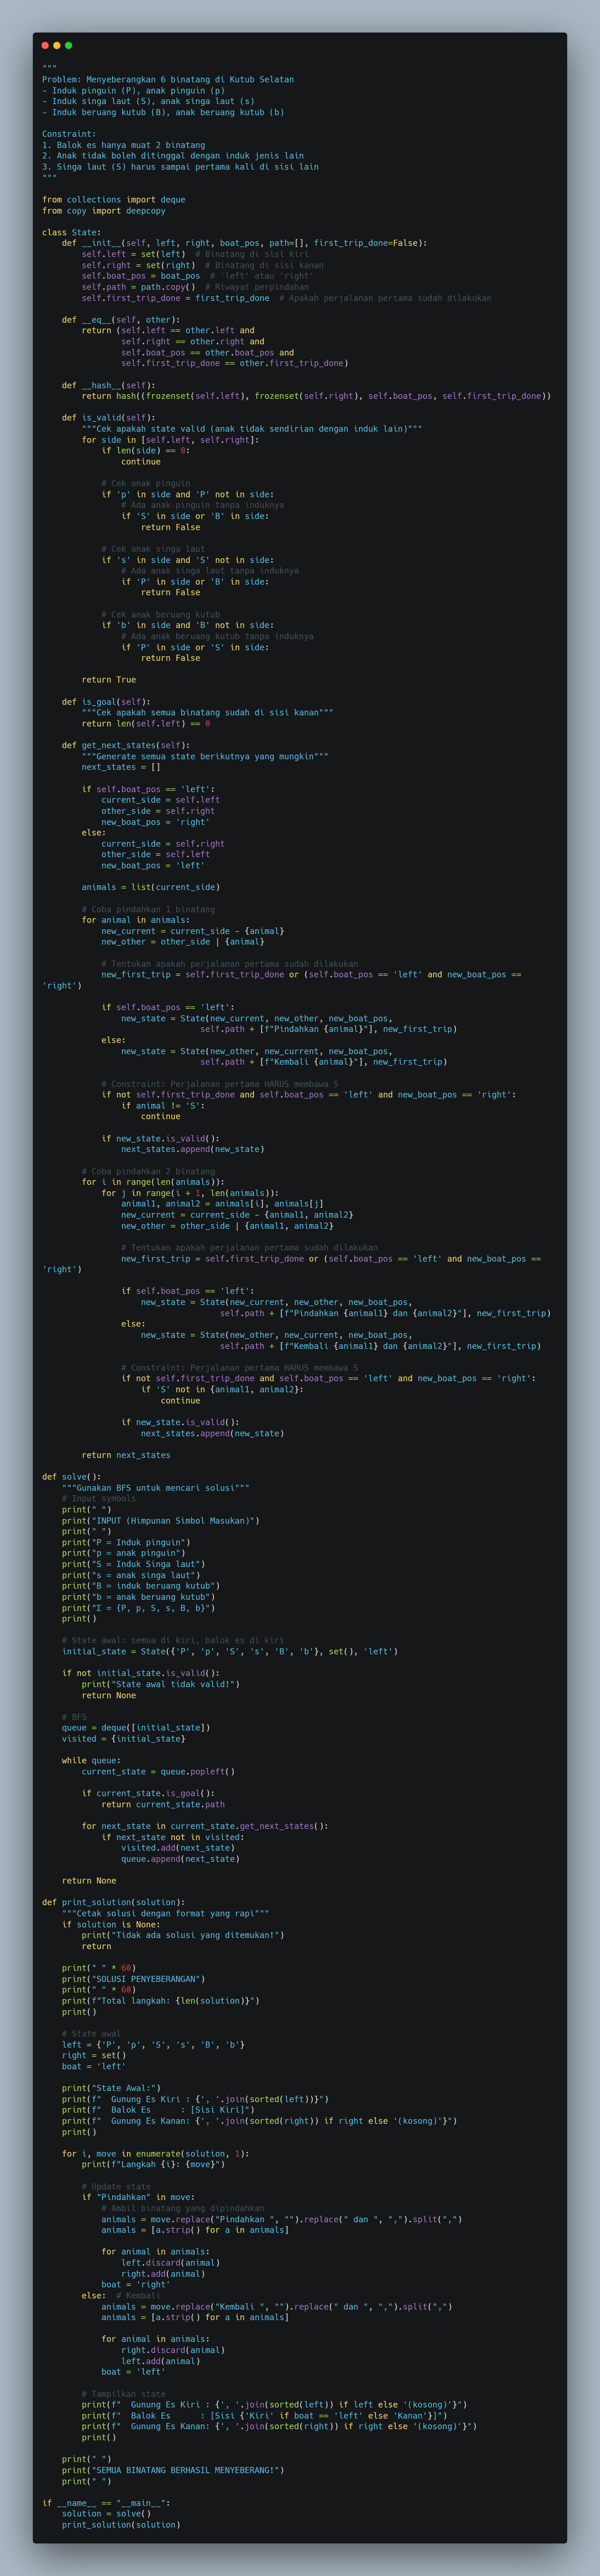
\includegraphics[width=0.8\textwidth]{code-python.png}
    \caption{Simulasi Penyeberangan Binatang dengan Python}
    \label{fig:simulation}
\end{figure}

\newpage

\begin{figure}[H]
    \centering
    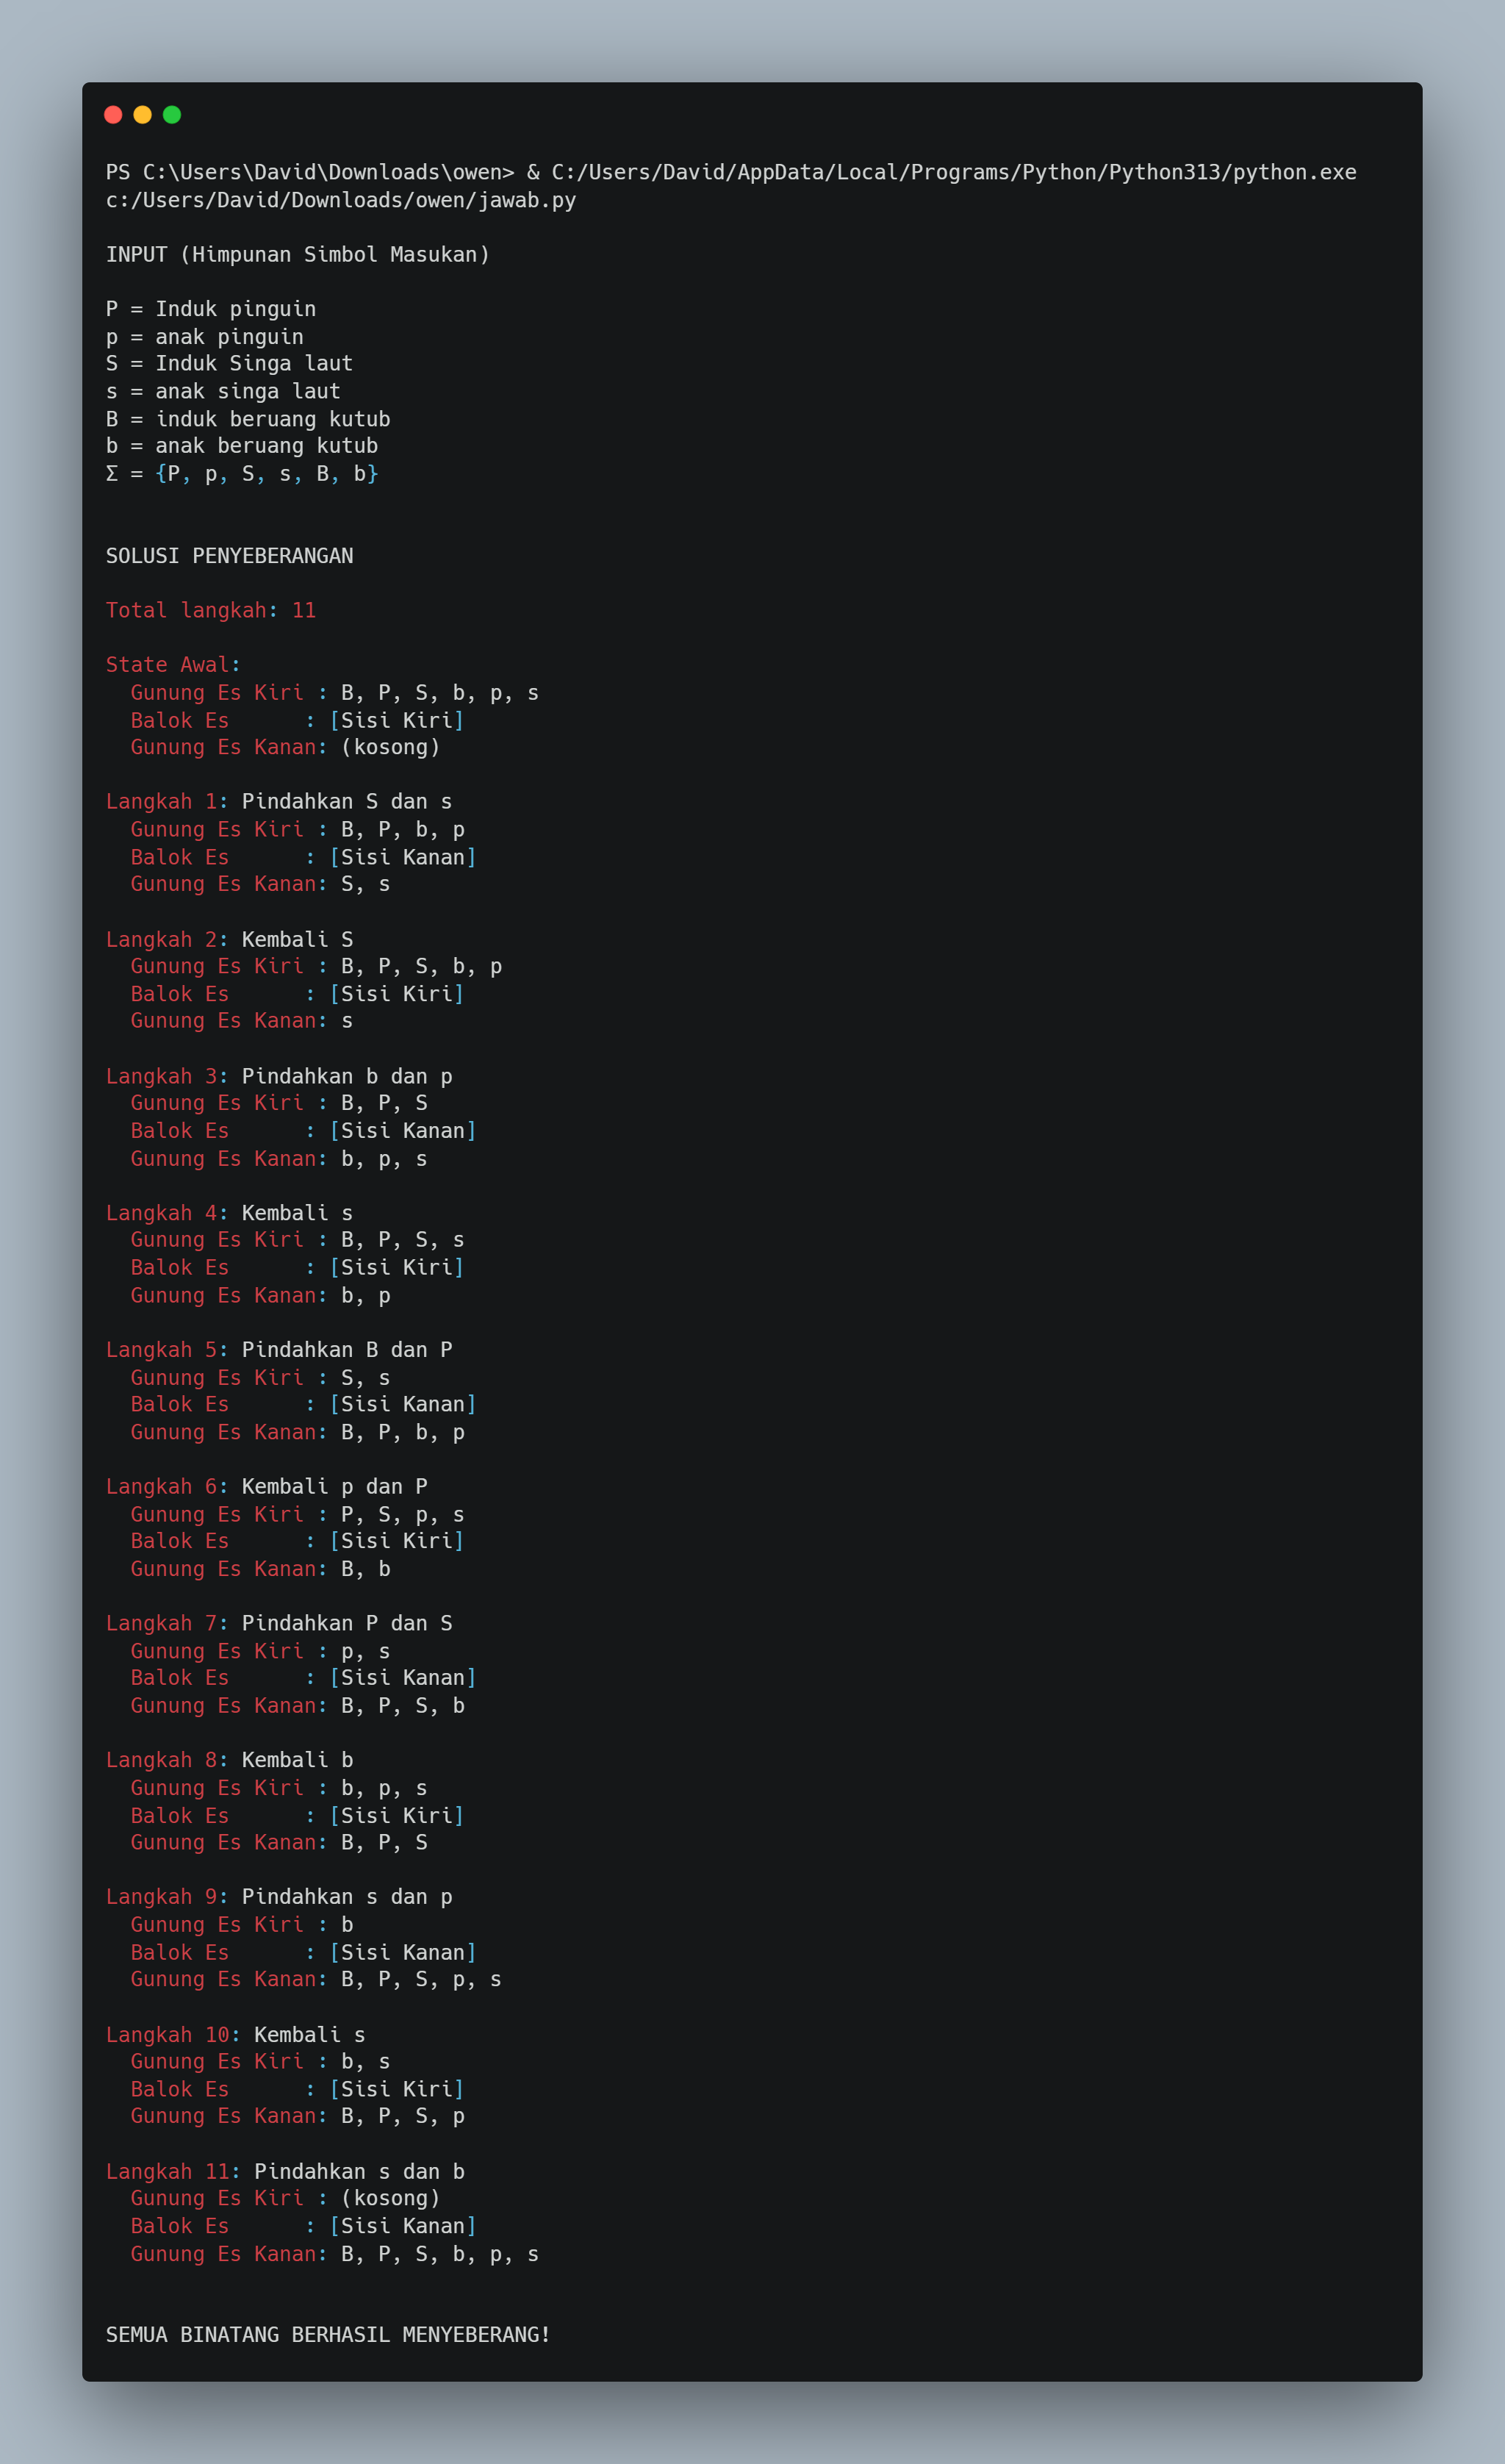
\includegraphics[width=0.8\textwidth]{output-python.png}
    \caption{Output Simulasi Penyeberangan Binatang dengan Python}
    \label{fig:output}
\end{figure}

\subsection*{JFLAP}
\begin{figure}[H]
    \centering
    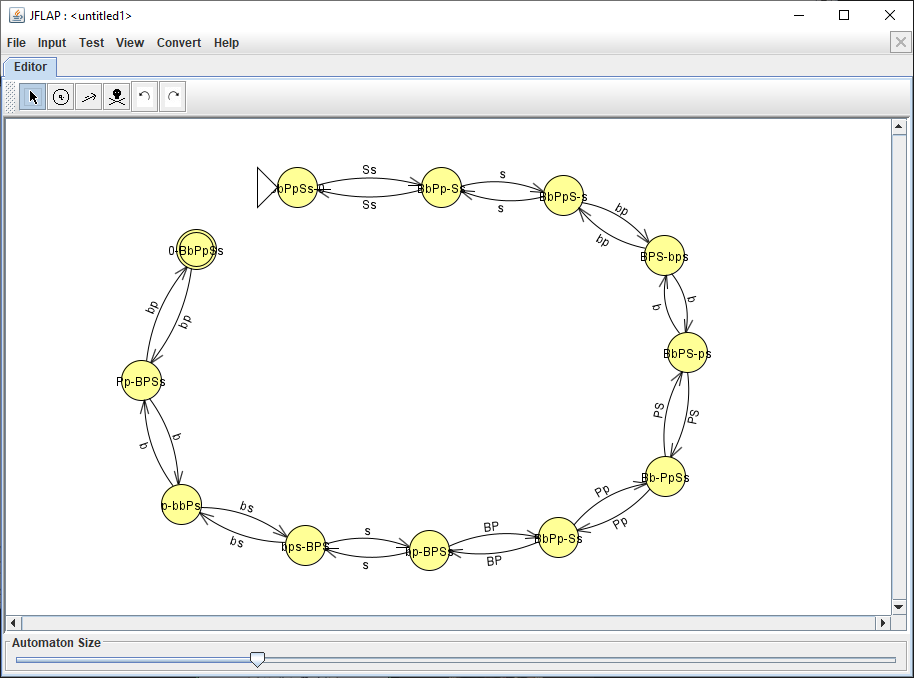
\includegraphics[width=1\textwidth]{jflap.png}
    \caption{Visualisasi Penyeberangan Binatang dengan JFLAP (Bagian 1)}
    \label{fig:jflap}
\end{figure}

\section*{Terminologi}
\begin{itemize}
    \item \textbf{State}: Kondisi atau situasi tertentu dalam proses penyeberangan binatang.
    \item \textbf{Transisi}: Perpindahan dari satu state ke state lainnya berdasarkan aturan yang telah ditentukan.
    \item \textbf{Notasi}: Simbol atau singkatan yang digunakan untuk mewakili binatang dalam proses penyeberangan.
\end{itemize}

\end{document}